\documentclass[9pt]{article}
\usepackage[utf8]{inputenc}
\usepackage[a4paper, margin=1cm]{geometry}
\usepackage{graphicx}
\usepackage[french]{babel}

% \usepackage[default,scale=0.30]{opensans}
\usepackage[T1]{fontenc}
\usepackage{amssymb} %math
\usepackage{amsmath}
\usepackage{amsthm}
\usepackage{systeme}
\usepackage{bbm}
\usepackage{hyperref}
\usepackage{multicol}
\usepackage{sectsty}
\usepackage{titlesec}


% \titleformat{\section}[runin]{\footnotesize\bfseries\sffamily}{\thesection}{1em}{}

% \titleformat{\subsection}[runin]{\footnotesize\bfseries\sffamily}{\thesubsection}{1em}{}[]
% \titleformat{\subsubsection}[runin]{\footnotesize\bfseries\sffamily}{\thesubsubsection}{1em}{}[]
% \titleformat{\paragraph}[runin]{\footnotesize\bfseries\sffamily}{\theparagraph}{1em}{}[]
% \titleformat{\subparagraph}[runin]{\footnotesize\bfseries\sffamily}{\thesubparagraph}{1em}{}[]

\titleformat{\section}[runin]{\normalfont\footnotesize\bfseries}{\thesection}{1em}{}
\titleformat{\subsection}[runin]{\normalfont\footnotesize\bfseries}{\thesubsection}{1em}{}
\titleformat{\subsubsection}[runin]{\normalfont\footnotesize\bfseries}{\thesubsubsection}{1em}{}
\titleformat{\paragraph}[runin]{\normalfont\footnotesize\bfseries}{\theparagraph}{1em}{}
\titleformat{\subparagraph}[runin]{\normalfont\footnotesize\bfseries}{\thesubparagraph}{1em}{}

\titlespacing*{\section}{0pt}{0.8mm}{0.1mm}
\titlespacing*{\subsection}{0pt}{0.1mm}{0.1mm}

\hypersetup{
    colorlinks=true,
    linkcolor=blue,
    filecolor=magenta,      
    urlcolor=cyan,
    pdftitle={LA FICHE},
    % pdfpagemode=FullScreen,
    }
\urlstyle{same} %\href{url}{Text}

\theoremstyle{plain}% default
\newtheorem{thm}{Théorème}[section]
\newtheorem{lem}[thm]{Lemme}
\newtheorem{prop}[thm]{Proposition}
\newtheorem*{cor}{Corollaire}
%\newtheorem*{KL}{Klein’s Lemma}

\theoremstyle{definition}
\newtheorem{defn}{Définition}[section]
\newtheorem{exmp}{Exemple}[section]
% \newtheorem{xca}[exmp]{Exercise}

\theoremstyle{remark}
\newtheorem*{rem}{Remarque}
\newtheorem*{note}{Note}
%\newtheorem{case}{Case}



\title{Liste des Tests du cours}
\author{Charles Vin}
\date{2022}

\begin{document}

\footnotesize
\begin{multicols}{3}

\section{KS d'adéquation}
\subsection*{Statistique de test} 
\begin{align*}
    h(F_n, F) &= \sup _{t \in \mathbb{R}} \left| F_n(t) - F(t) \right| \\
        &= \max _{1 \leq i \leq n} ( \max ( \left| \frac{i}{n} - F(X_{(i)}) \right| , \left| \frac{i-1}{n}- F(X_{(i)}) \right|  ))
\end{align*}    

\subsection*{Zone de Rejet}
\textbf{Si n est petit} table
\textbf{Si n est grand $ n \geq 30 $ }
\[
    \sqrt[]{n}h_n \to ^{\mathcal{L}}_{n \to \infty } W_{\infty }
.\]
\[
    \mathcal{R} = \{h(F_n, F_X) \geq \frac{k_\alpha }{\sqrt[]{n}} \}
.\]
$ k_{\alpha } $ le quantile de $ W_\infty $

\subsection*{Méthode}
Tableau avec i, $X_{(i)}$, $F_0(X_{(i)})$, $\frac{i}{n}$, $|\frac{i}{n} - F_0(X_{(i)})|$, $|\frac{i-1}{n} - F_0(X_{(i)})|$, 

\section{$ \mathcal{X}^2 $ d'ajustement}
\subsection*{Conditions}
Discret, n grand $ np_i \leq 5 $ 

\subsection*{Hypothèse}
$H_0 = p = p^{ref}$ VS $H_1 = p \neq p^{ref}$

\subsection*{Statistique de test}
$D(\bar{p_n}, p^{ref}) \sum_{k=1}^{d} \frac{(N_{k,n} - np_k^{ref})^2}{n p_k^{ref}}\to ^{\mathcal{L}}_{n \to \infty } \mathcal{X}^2(d-1)$

\subsection*{Méthode}
Tableau $ \bar{p}, p_i, np_i $ \textbf{fusion des classes}

\subsection{$ \mathcal{X}^2 $ d'ajustement famille paramétrique}
Comme avant mais $ \mathcal{X}^2(d-1-M) $, $ M $ nombre de paramètre estimé.

\section{KS d'homogénéité}
\subsection*{Conditions}
Ech. indep. ; fdr. continue $ F_X, F_Y $ 

\subsection*{Hypothèse}
$ H_0 $ : $ F_{X_1} = F_{Y_1} $ VS $ \neq  $ 

\subsection*{Statistique de test}
$\sup _{s \in \mathbb{R}} \left| \frac{1}{n}\sum_{i=1}^{n} \mathbbm{1}_{X_i \leq t} - \frac{1}{n}\sum_{j=1}^{n} \mathbbm{1}_{Y_j \leq t} \right| $

\subsection*{Zone de Rejet}
\textbf{n petit} Table
\textbf{n grand} 
        \[
            h_{n_1, n_2} = \sqrt[]{\frac{nm}{n+m}}h(F_n, G_n) \to ^{\alpha }_{n,m \to +\infty } W_\infty \text{ voir KS asymptotique}
        .\]
        zone de rejet $ \sqrt[]{\frac{n+m}{nm}}W_\infty  $ avec $ W_\infty  $ quantile $ W_\infty  $.

\subsection*{Méthode}
Même qu'un khi deux classique. $ Z_{(i)} = (X_i, Y_i) $ + tableau  $Z_{(i)}$, $F_n$, $G_n$, $h_{n_1, n_2}$ 

\section{$ \mathcal{X}^2 $ indépendance}
\subsection*{Donnée}
Ech appariés. Discret. $ X $ dans $ M $ cas, $ Y $ dans $ N $ cas   

\subsection*{Conditions}
Loi discrète. $ n $ grand $ E_{i,j} \leq 5$ 

\subsection*{Hypothèse}
Indépendance

\subsection*{Statistique de test}
$D = \sum_{m=1}^{M}\sum_{n=1}^{N}\frac{( N_{m,n} - \frac{N_{m, \centerdot} N_{\centerdot, n}}{T})^2}{\frac{N_{m, \centerdot} N_{\centerdot, n}}{T}}$

\subsection*{Zone de Rejet}
Sous $ H_0 $, $ D \to \mathcal{X}^2 ((M-1)(N-1)) $. Sous $ H_1 $, $ D \to +\infty  $

\subsection*{Méthode}
\begin{figure}[!h]
    \centering
    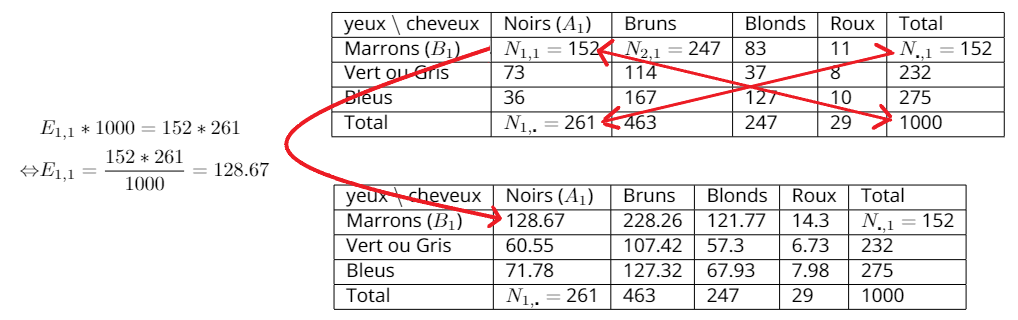
\includegraphics[width=.65\textwidth]{./src/fig1_test.png}
\end{figure}


\section{$ \mathcal{X}^2 $ d'homogénéité}
Deux ech. indep. à valeurs dans les mêmes classes $ A_1, \dots, A_M $. de vecteur loi  

\subsection*{Hypothèse}
On veut tester l'homogénéité : même vecteur loi ou pas

\section{Gaussiennes}
\subsection{Sur la moyenne}
\begin{itemize}
    \item Test sur 1 échantillon : Loi de Student \begin{itemize}
        \item Variance inconnu : On utilise $ \bar{X}_n $ dans $ V_n $ 
        \item Variance connu : on l'utilise à la place de $ V_n $ 
    \end{itemize}
    
    \item Test sur 2 échantillons indépendants : \begin{itemize}
        \item Variance inconnu : Test de welch : $ D = \frac{\bar{X}_{n_1} - \bar{Y}_{n_2}}{\sqrt[]{\frac{V_{n_1}^X}{n_1} + \frac{V_{n_2}^Y}{n_2}}} \sim_{H_0} \mathcal{T}(\mu ) $ avec $ \mu $ Formule horrible  
        \item Même variance inconnu : $ \bar{X}_{n_1} - \bar{Y}_{n_2} \sim \mathcal{N}(m_1 - m_2, \sigma ^2 (\frac{1}{n_1} + \frac{1}{n_2}))$ Same stat de test sauf qu'on estime la variance avec $ W = \frac{(n_1 - 1) V_{n_1}^X + (n_2 - 1) V_{n_2}^Y}{n_1 + n_2 - 2}$. Finalement la stat de test centrée réduite $ \sim \mathcal{T}(n_1 + n_2 - 2) $ 
        \item Variances connus :  $ \bar{X}_{n_1} - \bar{Y}_{n_2} \sim \mathcal{N}(m_1 - m_2, \sigma ^2 (\frac{1}{n_1} + \frac{1}{n_2}))$ cette fois-ci de variance connus
    \end{itemize}

    \item Test sur 2 échantillons appariés : $ Z_n = X_i - Y_i $ into $ \mathcal{T}(n-1) $ classique sur 1 échantillon  (Y'a un exo de td il parait)
\end{itemize}

\subsection{Sur la variance}
\begin{itemize}
    \item Test sur 1 échantillon : Comme le semestre d'avant \begin{itemize}
        \item Moyenne inconnu : On utilise $ \bar{X}_n $ dans le calcul de $ V_n $ puis penser que comme on connaît la moyenne ça suit une $ \mathcal{X}^2(n) $ 
        \item Moyenne connu : On l'utilise dans le calcul de $ V_n $ 
    \end{itemize}
    
    \item Test sur 2 échantillons indépendants : \begin{itemize}
        \item Moyenne inconnu : $ D = \frac{V_{n_1}^X}{V_{n_2}^Y} $ qui suit $ \mathcal{F}(n_1 - 1, n_2 - 1) $ sans besoin de transformation.
        \item Même Moyenne inconnu : X Pas de solution so do same as before
        \item Moyennes connus : L'utiliser dans les calcul des $ V_n $. Est-ce qu'on gagne des degrés de liberté ?
    \end{itemize}

    \item Test sur 2 échantillons apparié : X (maybe un Zn into khi deux)
\end{itemize}

\section{Somme des rangs}
\subsection*{Donnée}
Deux ech. indep. de fdr. cont.

\subsection*{Conditions}
Continue ; mieux que KS à 2 ech.

\subsection*{Hypothèse}
\begin{itemize}
    \item $ H_0 = X_1 $ et $ Y_1 $ ont la même loi. $ F_{X_1} = F_{Y_1} $ 
    \item $ H_0 = X_1 $ et $ Y_1 $ n'ont pas la même loi. $ F_{X_1} neq F_{Y_1} $ \begin{itemize}
        \item Ou $ X_1 \succ Y_1 $ C'est à dire $ F_{X_1} \neq F_{Y_1} $ et $ \forall t \in \mathbb{R}, F_{Y_1}(t) \leq F_{X_1}(t) $ 
        \item Ou $ Y_1 \succ X_1 $ C'est à dire $ F_{X_1} \neq F_{Y_1} $ et $ \forall t \in \mathbb{R}, F_{X_1}(t) \leq F_{Y_1}(t) $ 
    \end{itemize}
\end{itemize}

\subsection*{Statistique de test}
$U = \sum_{i=1}^{n_1}R(i) $ somme des rang des $ X_i $ 
\textbf{ex-æquo} rang moyen des rangs.

\subsection*{Zone de Rejet}
Utiliser symétrie.
\textbf{n grand} TCL

\subsection*{Méthode}
tableau obs de différente couleur.

\section{Signe}
\subsection*{Donnée}
Deux ech. apparié. + $ Z_i = Y_i - X_i $ médiane $ m_Z $ 

\subsection*{Conditions}
Fonction de répartition continue.

\subsection*{Hypothèse}
$ H_0 m_Z = 0 $ VS $ H_1 = m_Z \neq 0 $ ou autre possibilités

\subsection*{Statistique de test}
$S_n = \sum_{i=1}^{n}\mathbbm{1}_{Z_i \leq 0} = \text{ Nombre de } Y_i > X_i$ \textbf{d'ex-æquo} = rang moyen des rangs


\subsection*{Zone de Rejet}
\begin{itemize}
    \item Sous $ H_0 : P(Z_i > 0) = P(Y_i > X_i) = \frac{1}{2} \Rightarrow S_n \sim Bin(n,\frac{1}{2})$
    \item Sous $ H_1 $ \begin{itemize}
        \item Si $ m_z > 0, P(Y_i > X_i) > \frac{1}{2}, S_n \sim Bin(n,p), p> \frac{1}{2} $ donc $ S_n $ est "grand"
        \item Si $ m_z < 0, P(Y_i < X_i) > \frac{1}{2} $ donc $ S_n $ est petit.
        \item Si $ m_z \neq  0, S_n $ a un comportement proche des extremes (petit/grand).
    \end{itemize}
\end{itemize}
Table de la loi binomiale.\textbf{n grand} = TCL.


\section{Signe et Rang}
\subsection*{Donnée}
Deux ech. apparié. $ Z_i = Y_i - X_i $ iid. de médiane $ m $

\subsection*{Conditions}
La loi des $ Z_i $ est continue. Les $ Z_i $ sont symétriques par rapport à leur médiane $ m $.

\subsection*{Hypothèse}
$ H_0 = m = 0 \Leftrightarrow P(Y_i > X_i) = P(X_i < Y_i) = \frac{1}{2}$ VS $ H_0 = m \neq 0 $ ou $ m > 0 $ ou $ m < 0 $ 

\subsection*{Statistique de test}
Somme des rangs positif (ou négatif) des $ Z_{(i)} $

\subsection*{Zone de Rejet}
\begin{itemize}
    \item Sous $ H_0, W_n^+ \sim \mathcal{B}(n, \frac{1}{2}) $ 
    \item Sous $ H_1 $ \begin{itemize}
        \item $ H_1 : m > 0 \Leftrightarrow X_i > Y_i \Leftrightarrow $ plus de rang positif $ \Leftrightarrow W_n^+ $ prend de plus grande valeur et $ W_n^- $ de plus petite.
        \item $ H_1 : m > 0 $ Même raisonnement
        \item $ H_1 : m \neq 0 \Leftrightarrow W_n^+ $ prend des valeurs extremes.
    \end{itemize}
\end{itemize}
Bref on regarde la table avec le $ n $ nombre de couple $ (X_i, Y_i) $. On fait attention si on regarde $ W_n^+ $ ou $ W_n^- $. Et on utilise la symétrie avec les formules du centre ou des extrémités pour trouver l'autre quantile si besoin.
\subsection*{Méthode}
tableau $X_{(i)}$, $Y_{(i)}$, $Z_i$ , $Z_{(i)}$, Rang

\section{Indépendance Pearson}
\subsection*{Donnée}
Deux ech. apparié $ \mathcal{N}(m,\sigma ^2) $ 

\subsection*{Conditions}
Gaussien car c'est ce qui créé l'équivalence entre corrélation et indépendance

\subsection*{Hypothèse}
indépendance $\Leftrightarrow Cor = 0$

\subsection*{Statistique de test}
Soit $ R $ la corrélation empirique :
\begin{align*}
    R &= \frac{cov_n( (X_1, \dots, X_n), (Y_1, \dots, Y_n) )}{\sqrt[]{V_n^X*V_n^Y}} \\
    R_n &= \frac{\sum_{i=1}^{n} (X_i - \bar{X}_n) (Y_i - \bar{Y}_n)}{\sqrt[]{(\sum_{i=1}^{n} (X_i - \bar{X}_n)^2) \sum_{i=1}^{n} (Y_i - \bar{Y}_n)^2 }}
\end{align*}
\[
    D = \frac{R_n}{\sqrt[]{1 - R_n^2}} \sqrt[]{n-1}
.\]

\subsection*{Zone de Rejet}
Sous $ H_0, D \sim \mathcal{T}(n-2) $. Sous $ H_1, D $ est grand en valeur absolue

\section{Comparaison asymptotique de proportion}
\subsection*{Donnée}
Deux ech. indep. $ \mathcal{B}er(p_1 \text{ ou } p_2) $ 

\subsection*{Conditions}
Bernouilli + Ech indépendant

\subsection*{Hypothèse}
$ H_0 = p_1 = p_2 $ VS $ H_1 = p_1 \neq p_2 $ ou $ p_1 < p_2 $ ou $ p_1 > p_2 $ 

\subsection*{Statistique de test}
$S_{n,m} = \frac{\bar{X}_n - \bar{Y}_n}{\sqrt[]{ \frac{\bar{X}_n (1 - \bar{X}_n)}{n}} + \frac{\bar{Y}_n (1 - \bar{Y}_n)}{n}}$

\subsection*{Zone de Rejet}
\begin{itemize}
    \item Sous $ H_0, S_{n,m} \to ^\mathcal{L}_{n,m \to +\infty } \mathcal{N}(0,1)$
    \item Sous $ H_1 $ \begin{itemize}
        \item Si $ p_1 > p_2, S_{n,m} \to_{n,m \to \infty } +\infty  $ 
        \item Si $ p_1 < p_2, S_{n,m} \to_{n,m \to \infty } +\infty  $ 
        \item Si $ p_1 \neq  p_2, S_{n,m} \to_{n,m \to \infty } +\infty  $ 
    \end{itemize}
\end{itemize}
Donc
\begin{itemize}
    \item $ H_1 : p_1 > p_2, \mathcal{R} = \{S > h_{1 -\alpha }\} $ 
    \item $ H_1 : p_1 < p_2, \mathcal{R} = \{S > h_{\alpha }\} $ 
    \item $ H_1 : p_1 \neq  p_2, \mathcal{R} = \{S > h_{\alpha /2}\} \cup \{S > h_{1 - \alpha /2}\} $ 
\end{itemize}
Où les $ h_{\alpha } $ sont des quantiles de la loi normale.

\section{ANOVA}
\subsection*{Donnée}
$ K $ ech. gaussien de même variance

\subsection*{Conditions}
Échantillon gaussien indep., homoscédasticité : $ \sigma _1^2 = \dots = \sigma _K^2 $ 

\subsection*{Hypothèse}
égalité ou non des moyennes

\subsection*{Statistique de test}
$SCE^{totale}_{intra} = \sum_{p=1}^{K}SCE^{(p)}$ \\
$\bar{X} = \text{ moyenne totale } = \frac{1}{n}\sum_{p=1}^{K} n_p \bar{X}^{(p)}$ \\
$SCE_{inter} = \sum_{p=1}^{K} n_p (\bar{X}^{(p)} - \bar{X})^2$

\subsection*{Zone de Rejet}
$F = \frac{SCE_{inter} / (K-1)}{SCE_{intra}^{totale} / (n-K)}$
Sous $ H_0 : F \sim \mathcal{F}(K-1, n-K) $. Sous $ H_1, F $ prend de grande valeurs.

\subsection*{Méthode}
Tout calculer jusqu'à la stat de test. \begin{itemize}
    \item Si la loi de Fisher est trop grande. On se souvient que \begin{align*}
        &\frac{\mathcal{X}^2(k)}{k} \to _{k \to +\infty} 1 \\
        \Rightarrow & F = \frac{SCE_{inter} / (K-1)}{SCE_{intra}^{totale} / (n-K)} \to \frac{SCE_{inter} / (K-1)}{1} \\
        &= \mathcal{X}^2(K-1) / K-1
    \end{align*}
    \item Si on ne nous donne pas SCE directement on sait que
    \[
        SCE^{(p)} = \sum_{i=1}^{n_p} (X_i^{(p)} - \bar{X}^{(p)})^2 = (n_p -1) V^{(p)}
    .\]
\end{itemize}

\end{multicols}
\end{document}